\documentclass[a4paper, 12pt]{article}
\usepackage[T2A]{fontenc}
\usepackage[utf8]{inputenc}
\usepackage[english,russian]{babel}
\usepackage{amsmath, amsfonts, amssymb, amsthm, mathtools, misccorr, indentfirst, multirow}
\usepackage{wrapfig}
\usepackage{graphicx}
\usepackage{subfig}
\usepackage{adjustbox}
\usepackage{pgfplots}

\usepackage{geometry}
\geometry{top=20mm}
\geometry{bottom=20mm}
\geometry{left=20mm}
\geometry{right=20mm}
\newcommand{\angstrom}{\textup{\AA}}

\title{Лабораторная работа 5.5\\Компьютерная сцинтилляционная $\gamma$-спектроскопия}
\author{Нехаев Александр, гр. 654}
\date{\today}
\begin{document}
\maketitle
\tableofcontents
\section{Введение}
\paragraph{Цель работы:}
определить зависимость энергии и интенсивности гамма-линий от различных гамма источников и идентифицировать их.
\paragraph{В работе используются:}
сцинтиллятор, ФЭУ, предусилитель импульсов, высоковольтный блок питания для ФЭУ, АЦП, компьютер.
\subsection{Теоретическое введение}
\paragraph{Фотоэффект.}
Это процесс взаимодействия гамма-кванта с электроном, связанным с атомом, при котором электрону передается вся энергия гамма-кванта. При этом электрону сообщается кинетическая энергия $T_e=E_\gamma-I_i$, где $E_\gamma$ -- энергия гамма-кванта, $I_i$ -- потенциал ионизации $i$-той оболочки атома. Фотоэффект особенно существенен для тяжелых веществ, где он идет с заметной вероятностью даже при высоких энергиях гамма-квантов. В легких веществах фотоэффект становится заметен лишь при относительно небольших энергиях гамма-квантов. Наряду с фотоэффектом, при котором вся энергия гамма-кванта передается атомному электрону, взаимодействие гамма-излучения со средой может приводить к его рассеянию, т.е. отклонению от первоначального направления распространения на некоторый угол.
\paragraph{Эффект Комптона.} Это упругое рассеяние фотона на свободном электроне, сопровождающееся изменением длины волны фотона (реально этот процесс происходит на слабо связанных с атомом внешних электронах). Максимальная энергия образующихся комптоновских электронов соответствует рассеянию гамма-квантов на $180^\circ$ и равна
\begin{equation}
E_{\max}=\frac{\eta\omega}{1+\frac{mc^2}{2\eta\omega}}.
\end{equation}
\paragraph{Процесс образования электрон-позитронных пар.}
При достаточно высокой энергии гамма-кванта наряду с фотоэффектом и эффектом Комптона может происходить третий вид взаимодействия гамма-квантов с веществом -- образование электрон-позитронных пар. Процесс образования пар не может происходить в пустоте, так как в этом случае не выполняются законы сохранения энергии и импульса. В присутствии ядра или электрона процесс образования пары гамма-квантом возможен, так как можно распределить энергию и импульс гамма-кванта между тремя частицами без противоречия с законами сохранения. При этом если процесс образования пары идет в кулоновском поле ядра или протона, то энергия образующегося ядра отдачи оказывается весьма малой, так что пороговая энергия гамма-кванта $E_0$, необходимая для образования пары, практически совпадает с удвоенной энергией покоя электрона $E_0\cong 2mc^2=1.022$ МэВ.\par
Появивишийся в результате процесса образования пар электрон свою энергию на ионизацию среды. Таким образом, вся энергия электрона остается в детекторе. Позитрон будет двигаться до тех пор, пока практически не остановится, а затем аннигилирует с электроном среды, в результате чего появятся два гамма-кванта. Т.е., кинетическая энергия позитрона также останется в детекторе. Далее возможны три варианта развития событий:
\begin{enumerate}
\item оба родившихся гамма-кванта не вылетают из детектора, и тогда вся энергия первичного гамма-кванта останется в детекторе, а в спектре появится пик с $E=E_{\gamma}$;
\item один из родившихся гамма-квантов покидает детектор, и в спектре появляется пик, соответствующий энергии $E=E_{\gamma}-E_0$, где $E_0=mc^2=511$ кэВ;
\item оба родившихся гамма-кванта покидают детектор, и в спектре появляется пик, соотвествующий энергии $E=E_{\gamma}-2E_0$, где $2E_0=2mc^2=1022$ кэВ.
\end{enumerate}
Таким образом, любой спектр, получаемый с помощью гамма-спектрометра, описывается несколькими компонентами, каждая из которых связана с определенным физическим процессом. Как описано выше, основными физическими процессами взаимодействия гамма-квантов с веществом является фотоэффект, эффект Компотона и образование электрон-позитронных пар, и каждый из них вносит свой вклад в образование спектра. Помимо этих процессов, добавляется экспонента, связанная с наличием фона, пик характеристического излучения, возникающий при взаимодействии гамма-квантов с окружающим веществом, а также пик обратного рассеяния, образующийся при энергии квантов $E_{\gamma}\gg mc^2/2$ в результате рассеяния гамма-квантов на большие углы на материалах  конструктивных элементов детектора и защиты. Положение пика обратного рассеяния определяется по формуле:
\begin{equation}
E_{\text{обр}}=\frac{E}{1+2E/mc^2},
\label{eq:Ereverse}
\end{equation}
где $E$ -- энергия фотопика.\par
\paragraph{Энергетическое разрешение спектрометра.} Даже при поглощении частиц с одинаковой энергией амплитуда импульса на выходе фотоприёмника сцинтилляционного детектора меняется от события к событию. Это связано:
\begin{enumerate}
\item со статистическим характером процессов сбора фотонов на фотоприёмнике и последующего усиления,
\item с различной вероятностью доставки фотона к фотоприемнику из разных точек сцинтиллятора,
\item с разбросом высвечиваемого числа фотонов
\end{enumerate}
\par
В результате в набранном спектре линия (которая для идеального детектора представляла бы дельта-функцию) оказывается размытой, её часто описывают гауссианом.\par
Энергетическим разрешением спектрометра называется величина
\begin{equation}
R_i=\frac{\Delta E_i}{E_i},
\end{equation}
где $\Delta E_i$ -- ширина пика полного поглощения, измеренная на половине высоты, $E_i$ -- энергия регистрируемого $\gamma$-излучения. Значение $E_i$ пропорционально среднему числу фотонов $\overline{n_i}$ на выходе ФЭУ, т.е.:
\begin{equation}
E_i=\alpha\overline{n_i}.
\label{eq:4}
\end{equation}
\par
Полуширина пика полного поглощения $\Delta E_i$ пропорциональна среднеквадратичной флуктуации $\overline{\Delta n_i}$. Т.к. $n_i$ является дискретной случайной величиной, которая распределена по закону Пуассона, то $\overline{\Delta n_i}=\sqrt{\overline{n_i}}$ и поэтому
\begin{equation}
\Delta E_i=\alpha\overline{\Delta n_i}=\alpha\sqrt{\overline{n_i}}.
\label{eq:5}
\end{equation}
\par
Из (\ref{eq:4}), (\ref{eq:5}) получаем, что
\begin{equation}
R_i=\frac{\Delta E_i}{E_i}=\frac{\text{const}}{\sqrt{E_i}}.
\label{eq:6}
\end{equation}
\par
Поскольку энергетическое разрешение зависит от энергии, его следует указывать для конкретной энергии. Чаще всего разрешение указывают для энергии гамма-линии $^{137}\text{Cs}$ (661.7 кэВ).
\section{Ход работы}
Используем спектр $^{22}\text{Na}$ как калибровочный график:
\begin{figure}[!htb]
\centering
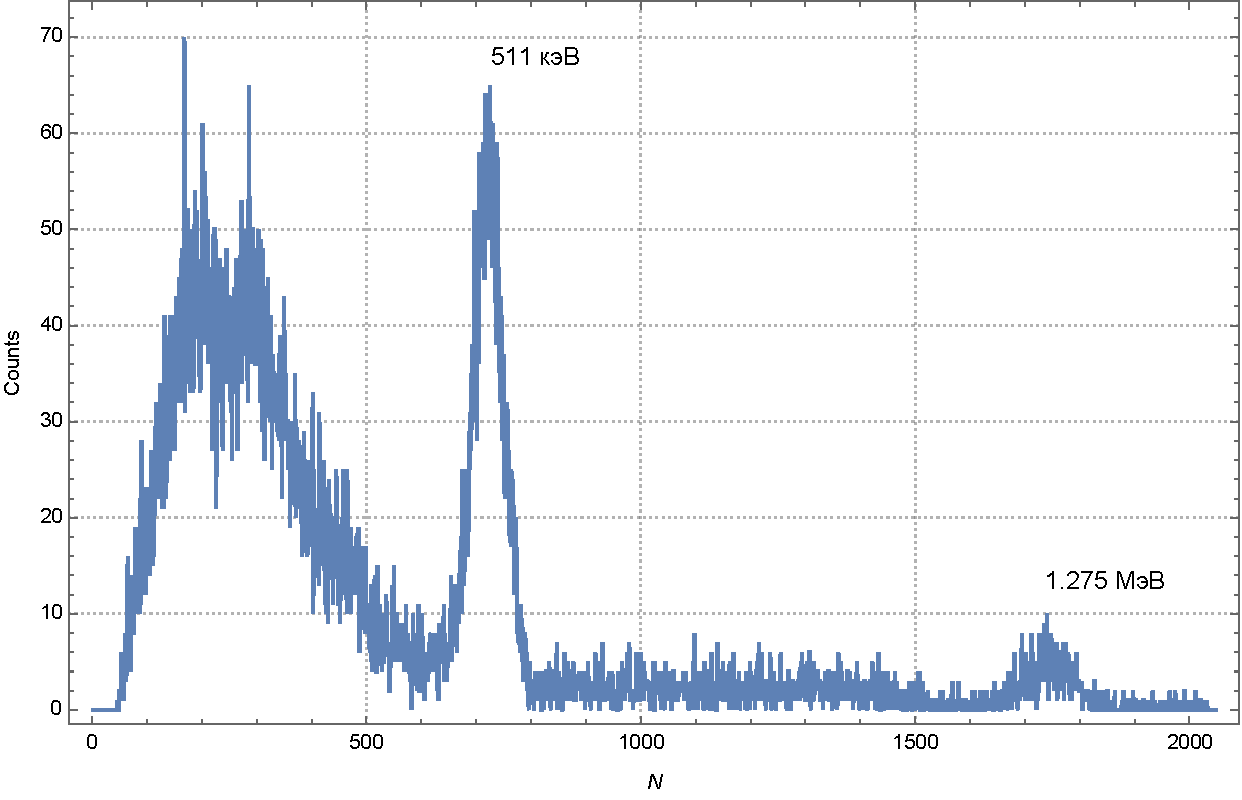
\includegraphics[scale=0.7]{calibration.pdf}
\caption{Спектр $^{22}$Na}
\end{figure}
\par
Построим калибровочный график зависимости номера канала $N$ от энергии $\gamma$-кванта $E_i$. Предварительно аппроксимируем пики по функции Гаусса:
\begin{equation}
y(x)=A\cdot e^{-\frac{(x-x_0)^2}{2*\sigma^2}}+B\cdot x+C
\end{equation}
Таким образом, спектр с аппроксимированными пиками имеет следующий вид:
\begin{figure}[!htb]
\centering
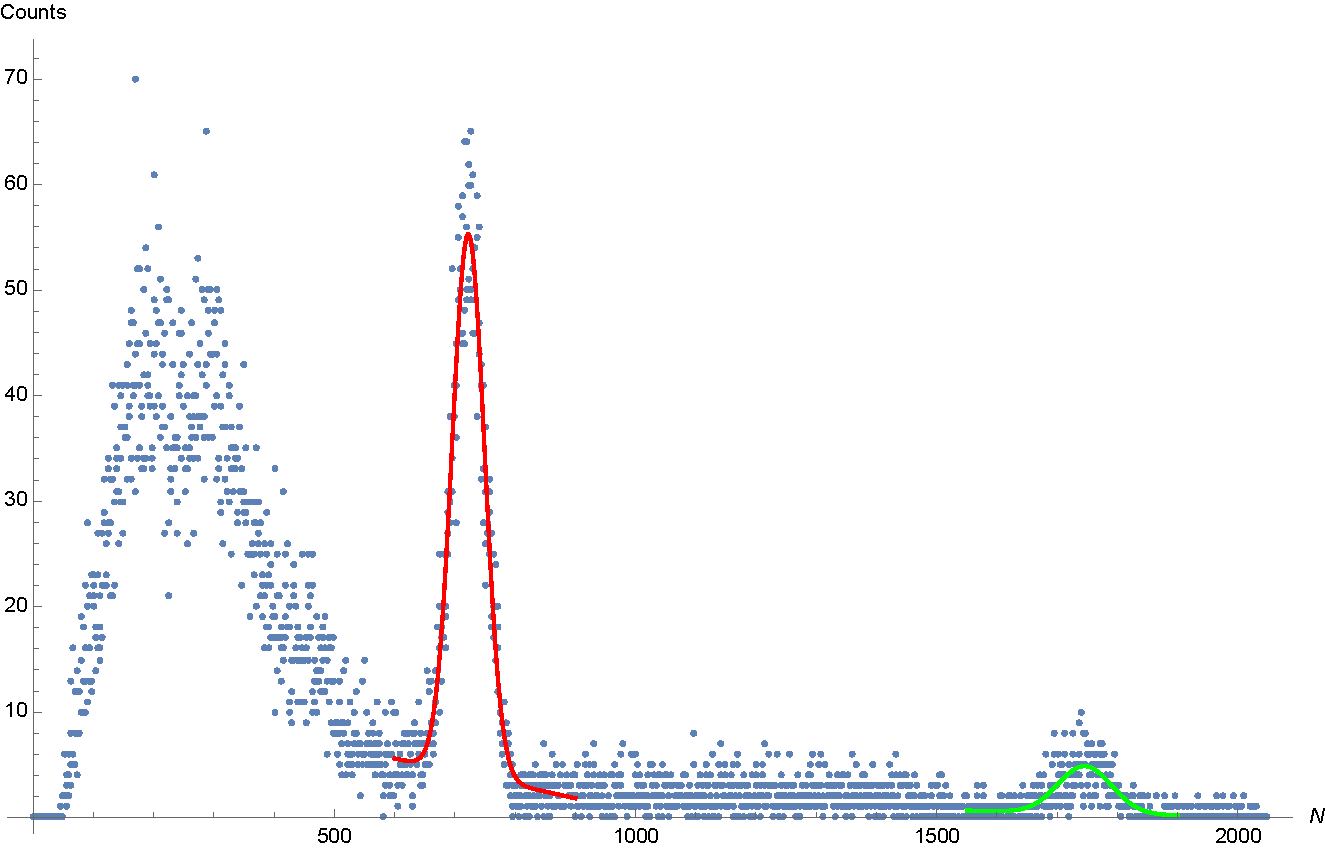
\includegraphics[scale=0.65]{calibration_approx.pdf}
\caption{Спектр $^{22}$Na с аппроксимированными пиками}
\end{figure}
\par
Координаты пиков по горизонтальной оси соответсвтуют параметру $x_0$. Для данных пиков: $x_{01}=722.438$, $x_{02}=1746$. Тогда калибровочный график имеет вид:
\begin{figure}[!htb]
\centering
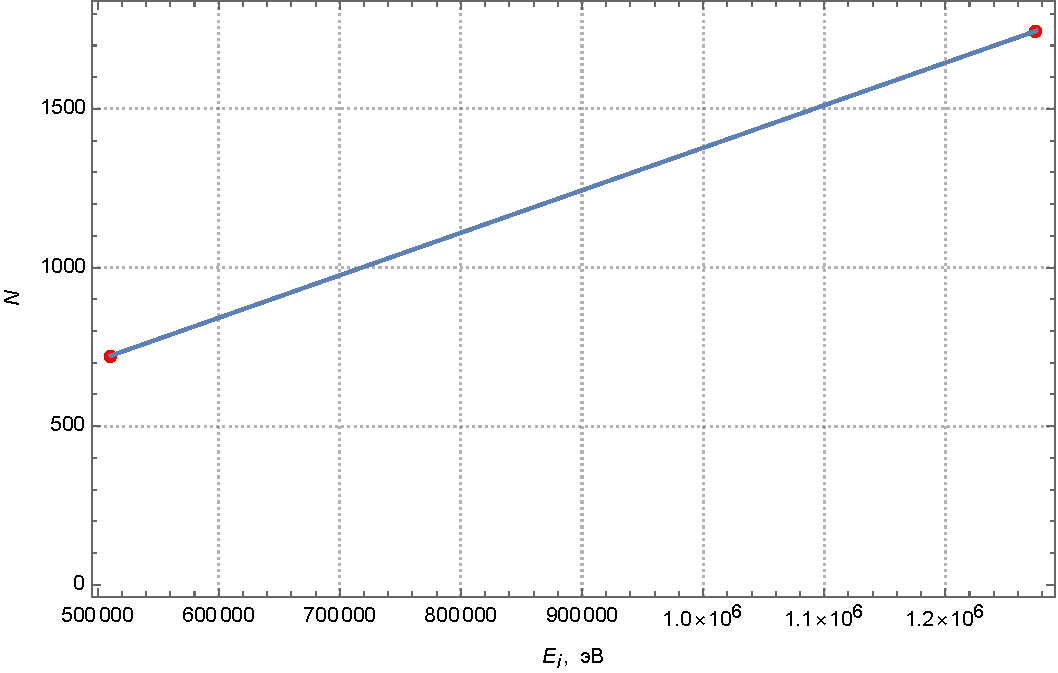
\includegraphics[scale=0.7]{calibrator.pdf}
\caption{Калибровочный график}
\end{figure}
\par
Функция для перевода номера канала в энергию имеет вид:
\begin{equation}
E_i=-28239.5 + 746.416\cdot N
\end{equation}
Используя калибровочный график, определим для всех остальных источников значения энергии пиков полного поглощения $E_i$, их ширины на половине высоты $\Delta H_i$ и энергетическое разрешение $R_i$.
\begin{figure}[!htb]
\centering
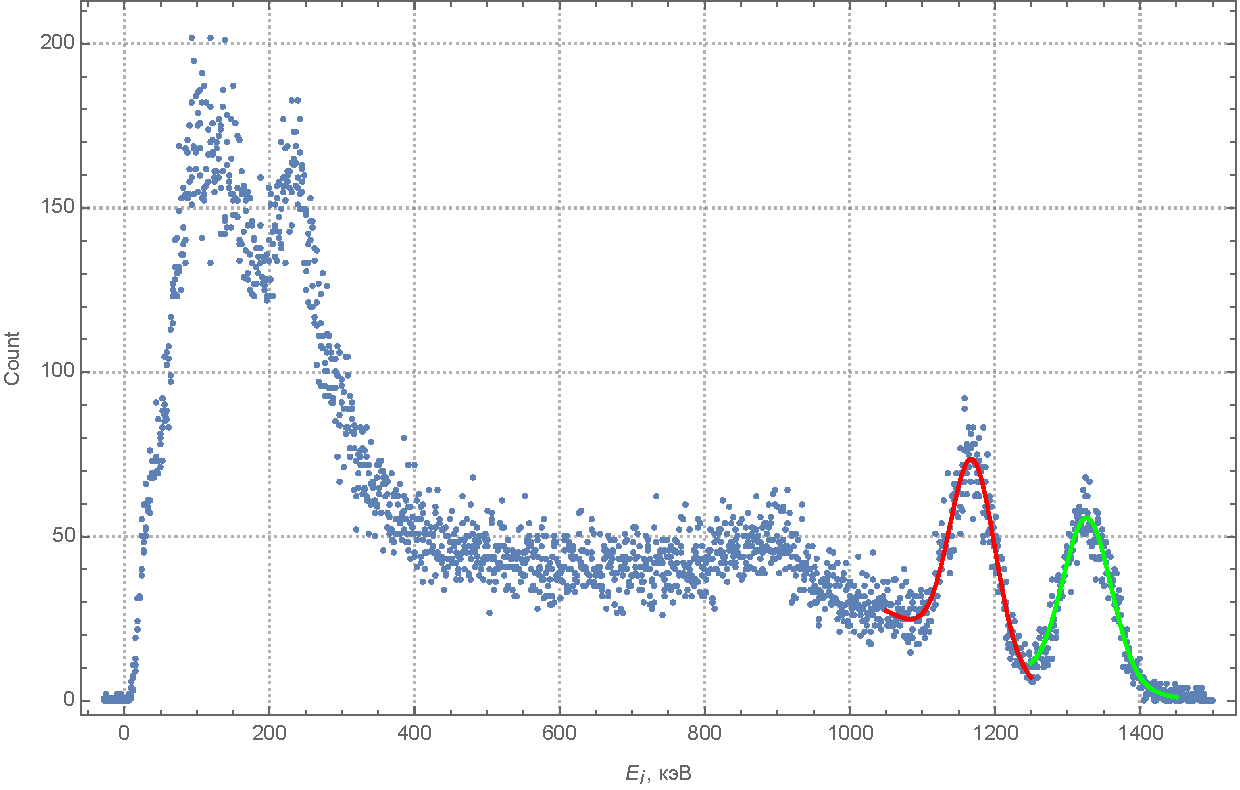
\includegraphics[scale=0.73]{co60.pdf}
\caption{Спектр $^{60}\text{Co}$}
\end{figure}
\begin{figure}[!htb]
\centering
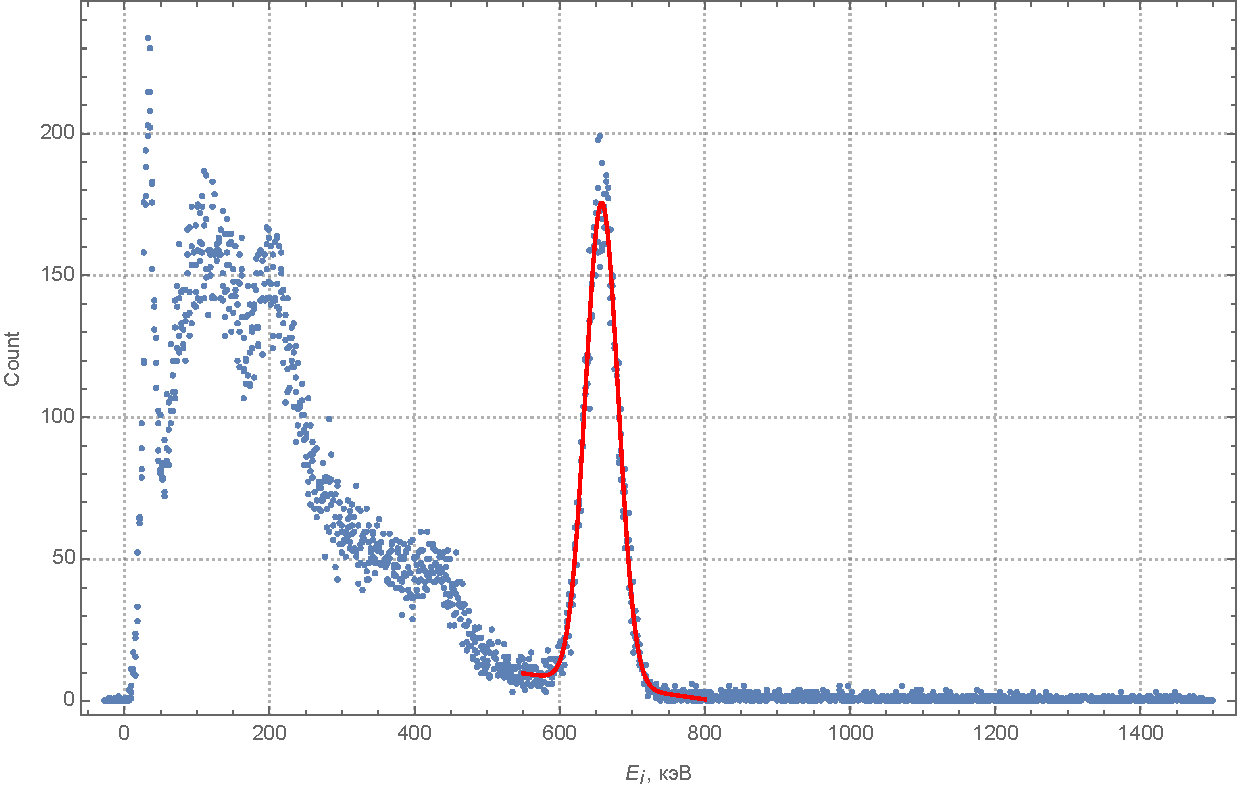
\includegraphics[scale=0.65]{cs137.pdf}
\caption{Спектр $^{137}\text{Cs}$}
\end{figure}
\begin{figure}[!htb]
\centering
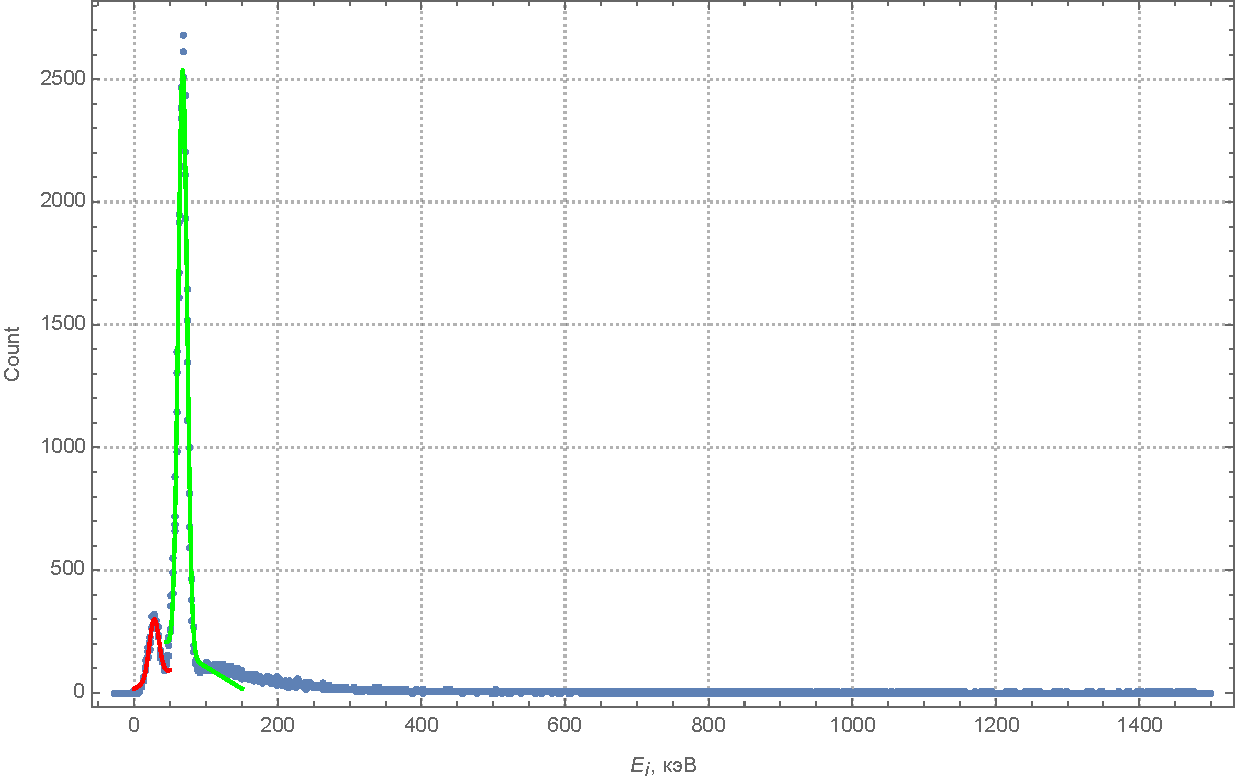
\includegraphics[scale=0.7]{am241.pdf}
\caption{Спектр $^{241}\text{Am}$}
\end{figure}
\begin{figure}[!htb]
\centering
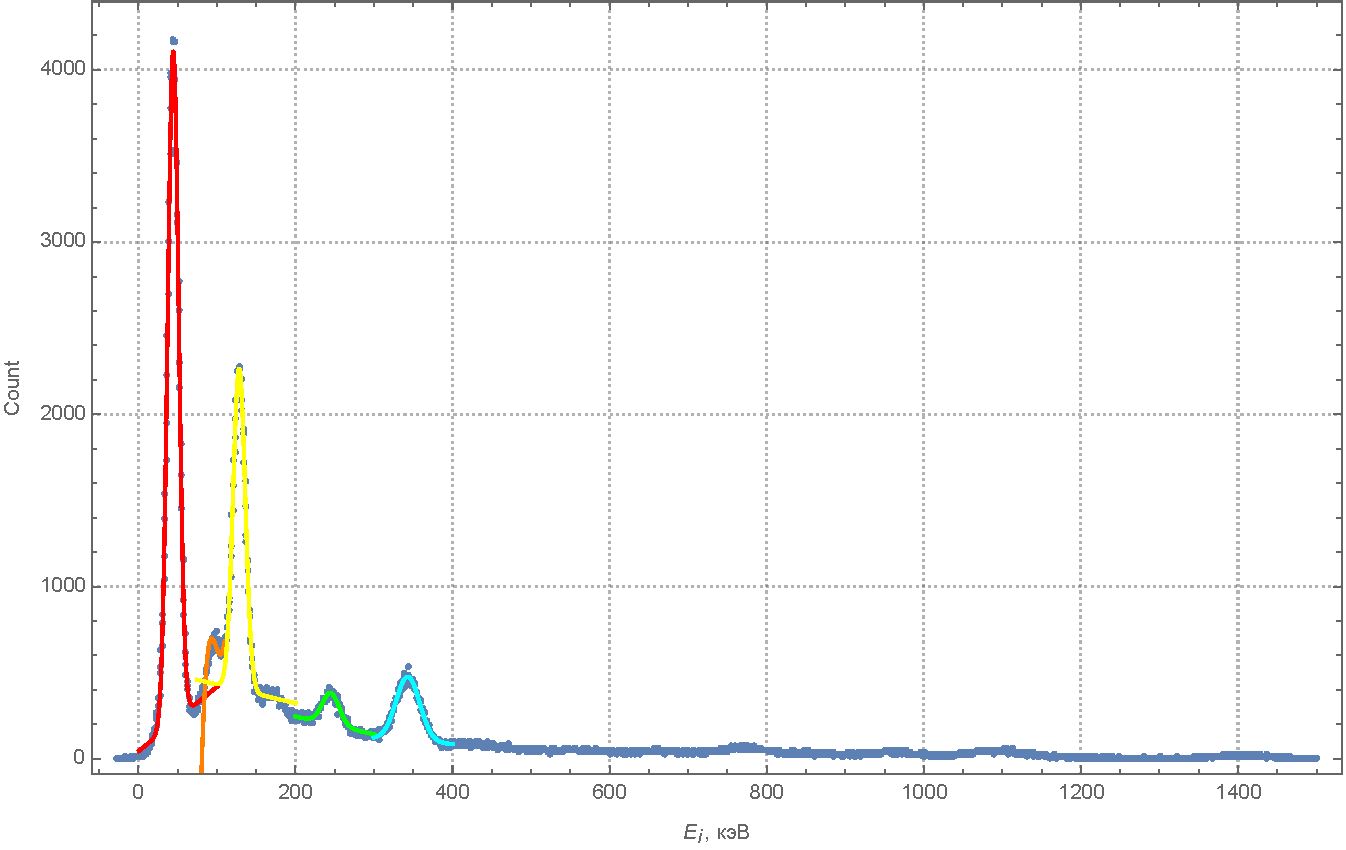
\includegraphics[scale=0.7]{eu152.pdf}
\caption{Спектр $^{152}\text{Eu}$}
\end{figure}
\newpage
\newpage
Сведем результаты в таблицу \ref{table1}.
\begin{table}[!htb]
\centering
\caption{Параметры пиков спектров}
\begin{tabular}{|c|c|c|c|c|c|}
\hline
Источник & $N_i$ & $\Delta N_i$ & $E_i$ & $\Delta E_i$ & $R_i$ \\
\hline
Cobalt & 1604 & 135 & $1169.01\text{keV}$ & $72.3899\text{keV}$ & 0.061924 \\
Cobalt & 1816 & 143 & $1327.06\text{keV}$ & $78.2396\text{keV}$ & 0.0589571 \\
Cesium & 919 & 109 & $658.017\text{keV}$ & $52.9515\text{keV}$ & 0.0804713 \\
Americium & 75 & 59 & $27.739\text{keV}$ & 1$5.8365\text{keV}$ & 0.570911 \\
Americium & 128 & 57 & $67.4993\text{keV}$ & $14.4587\text{keV}$ & 0.214205 \\
Europium & 97 & 60 & $44.4872\text{keV}$ & $16.5465\text{keV}$ & 0.371939 \\
Europium & 138 & 113 & $75.\text{keV}$ & $56.1468\text{keV}$ & 0.748624 \\
Europium & 210 & 62 & $128.477\text{keV}$ & $18.3269\text{keV}$ & 0.142648 \\
Europium & 366 & 72 & $245.012\text{keV}$ & $25.2028\text{keV}$ & 0.102864 \\
Europium & 498 & 85 & $343.194\text{keV}$ & $35.4755\text{keV}$ & 0.103368 \\
\hline
\end{tabular}
\label{table1}
\end{table}
В этой таблице: $N_i$ -- номер канала, соответствующего пику полного поглощения.\par
По результатам измерения энергии края комптоновского поглащения построим график, по одной оси которого отложены экспериментальные значения, а по другой расчетные значения этой энергии (рис. \ref{compton}).\par
\begin{figure}
\centering
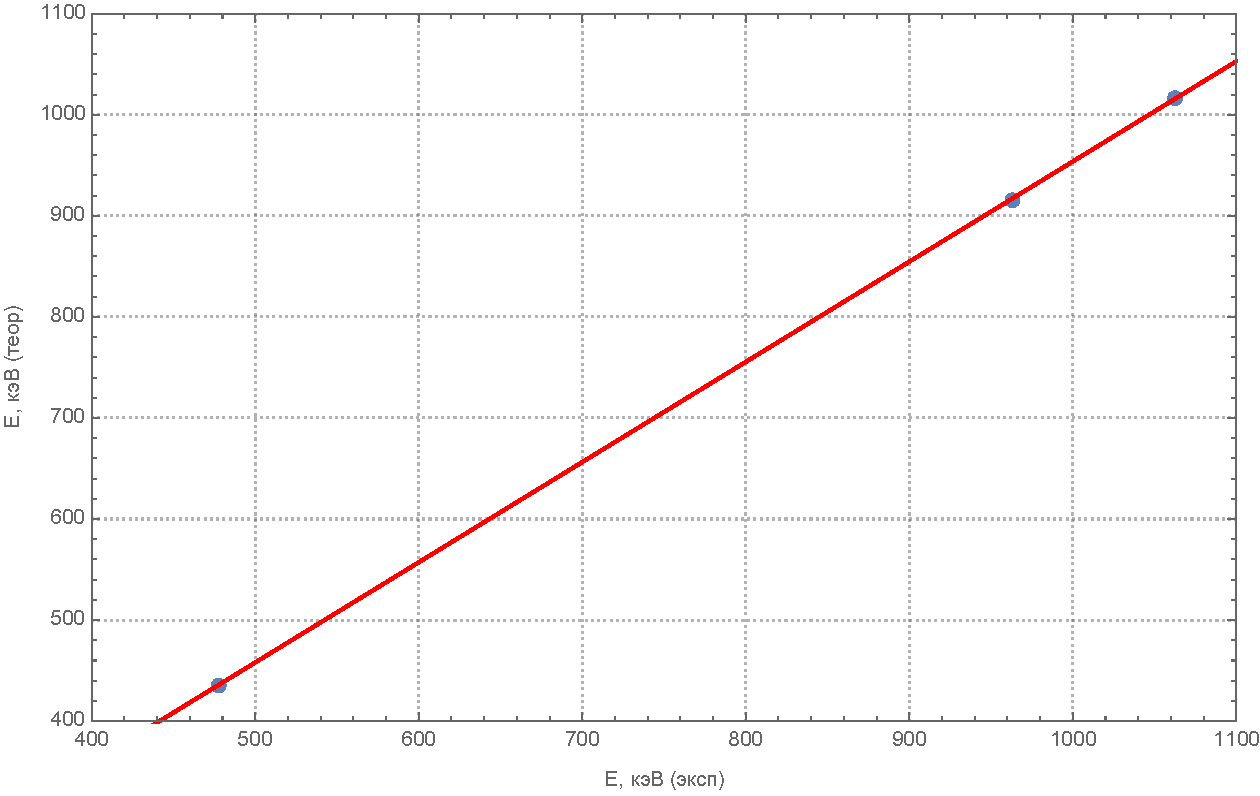
\includegraphics[scale=0.5]{edges.pdf}
\caption{Комптоновские края}
\label{compton}
\end{figure}
Для проверки зависимости (\ref{eq:6}), построим по полученным данным график $R_i^2=f\left(1/E_i\right)$ (рис. \ref{fig:re}).
\begin{figure}[!htb]
\centering
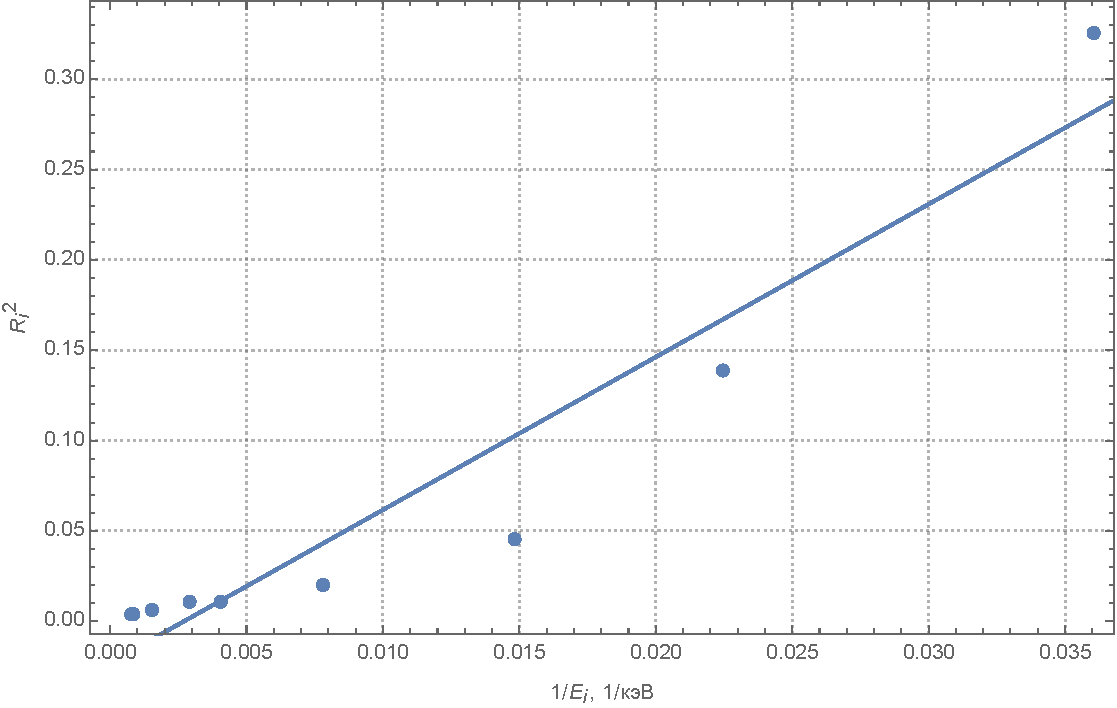
\includegraphics[scale=0.7]{Re.pdf}
\caption{Зависимость разрешения от энергии}
\label{fig:re}
\end{figure}
\par
Форма импульсов на выходе ФЭУ определяется выражением:
\begin{equation}
U(t)=\text{const}\cdot e^{-\frac{t}{RC}}\left(1-e^{-\frac{t}{\tau_0}}\right),
\label{eq:7}
\end{equation}
где $\tau_0$ -- время высвечивания сцинтиллятора, а $RC$ -- постоянная времени ($R$ и $C$ -- сопротивление и емкость в анодной цепи ФЭУ). Выражение (\ref{eq:7}) справедливо при $RC\gg\tau_0$. Обычно выбирают $RC=(5\div 10)\tau_0$. По зарисованным импульсам оценим величину $\tau_0$ и постоянную времени $RC$.
\begin{figure}[!htb]
\centering
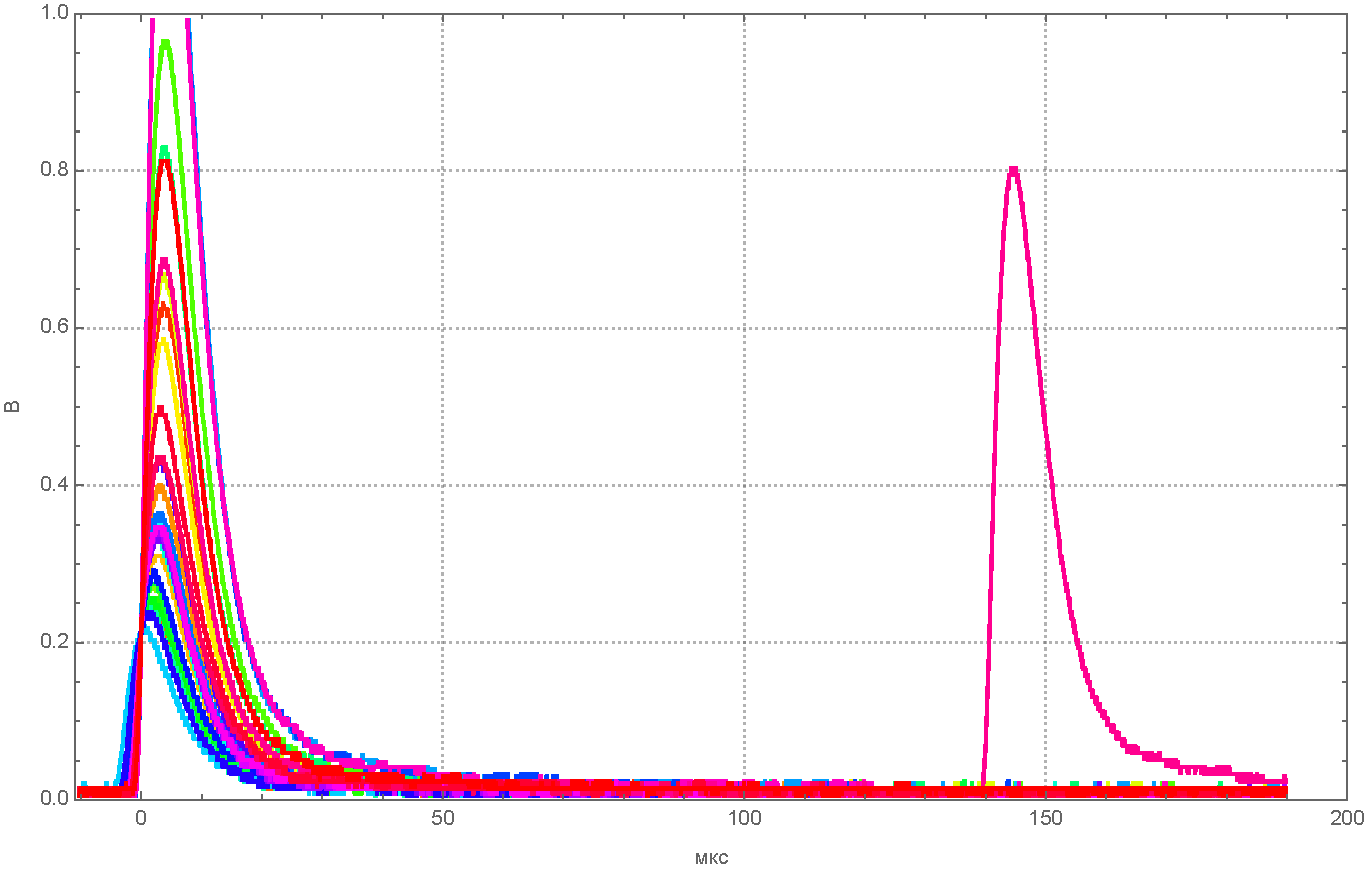
\includegraphics[scale=0.7]{oscil.pdf}
\caption{Форма импульса}
\end{figure}
\par
Аппроксимируя положительную часть графика согласно формуле (\ref{eq:7}), получаем, что $RC\approx 6.244 \mu s$, а $\tau_0\approx 3.61 \mu s$.\par
Построим график зависимости энергии пика обратного рассеяния от энергии.\par
Формула для определения энергии пика (\ref{eq:Ereverse}) применима для тех элементов, у которых $E_\gamma$ меньше $mc^2$. Этому условию удовлетворяют только два элемента: кобальт и цезий.
На графике для цезия, пик виден достаточно четко. На графике для кобальта пика должно быть два. Исходя из известных энергий фотопиков находим примерное положение пиков обратного рассеяния:
\begin{table}[!htb]
\centering
\caption{Примерное положение пиков обратного рассеяния}
\begin{tabular}{|c|c|c|}
\hline
Элемент & $E_\text{фотопика}$ & $E_\text{пика обратного рассеяния}$\\
\hline
$^{60}$Co & 1169.01\text{keV} & 209.673\text{keV} \\
$^{60}$Co & 1327.06\text{keV} & 214.25\text{keV} \\
$^{137}$Cs & 658.017\text{keV} & 184.039\text{keV} \\
\hline
\end{tabular}
\label{tab:peakapprox}
\end{table}
\par
Видим что расчетные энергии двух пиков кобальта отличаются всего на 4.5 кэВ. На графике эти два пика неразличимы. Аппрокимируем пик на графике кобальта (рис. \ref{fig:co60Re}). Аналагично аппроксимируем пик на графике цезия (рис. \ref{fig:ce137Re}).
\begin{figure}[!htb]
\centering
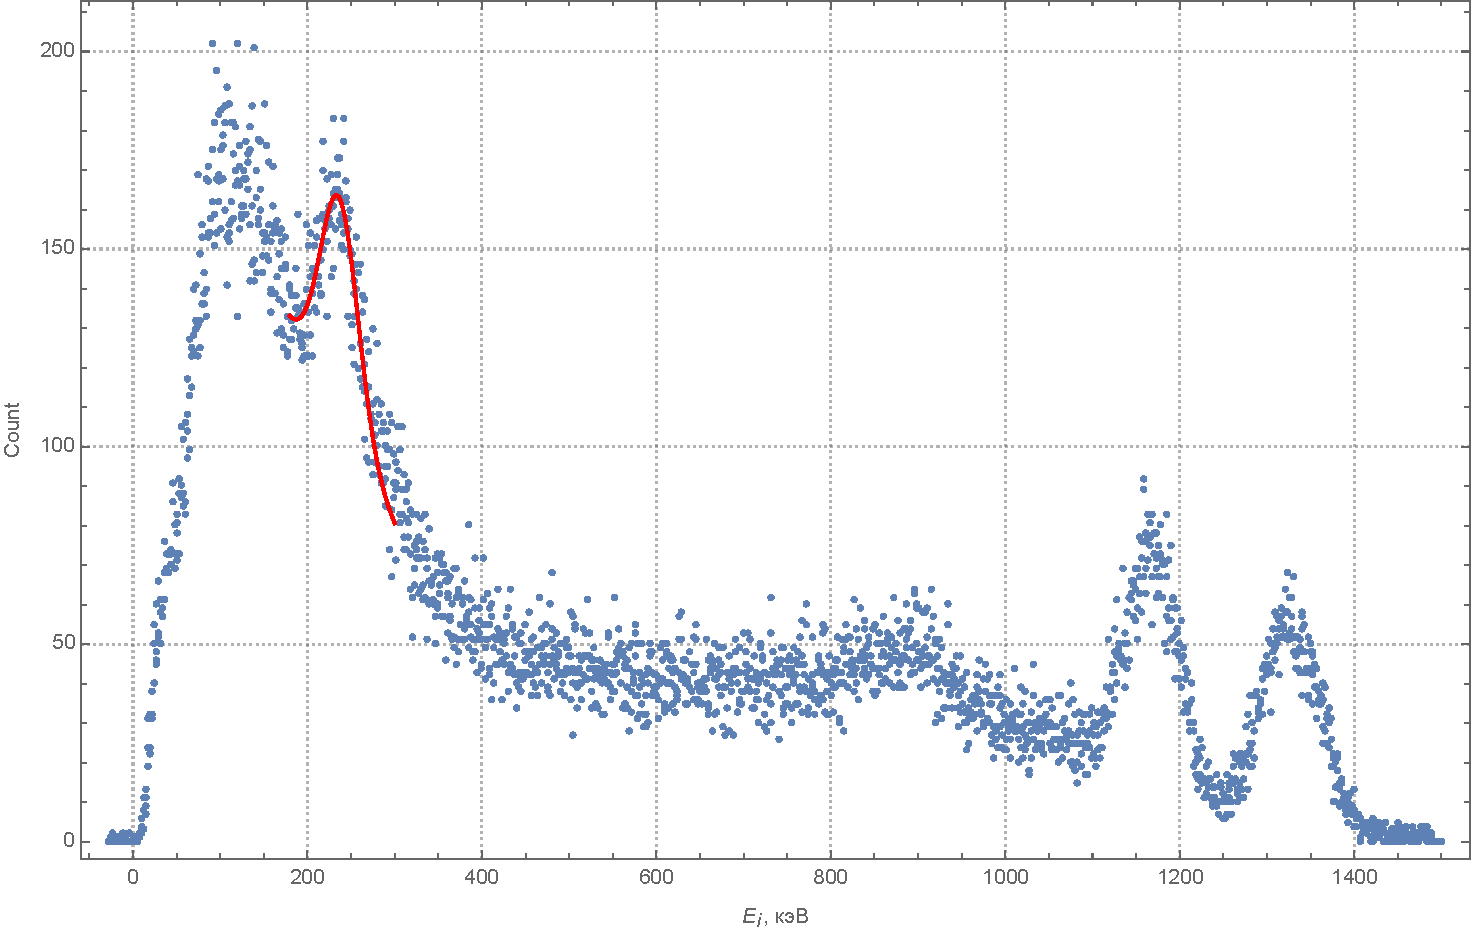
\includegraphics[scale=0.45]{co60Reverse.pdf}
\caption{Пик обратного рассеяния кобальта}
\label{fig:co60Re}
\end{figure}
\begin{figure}[!htb]
\centering
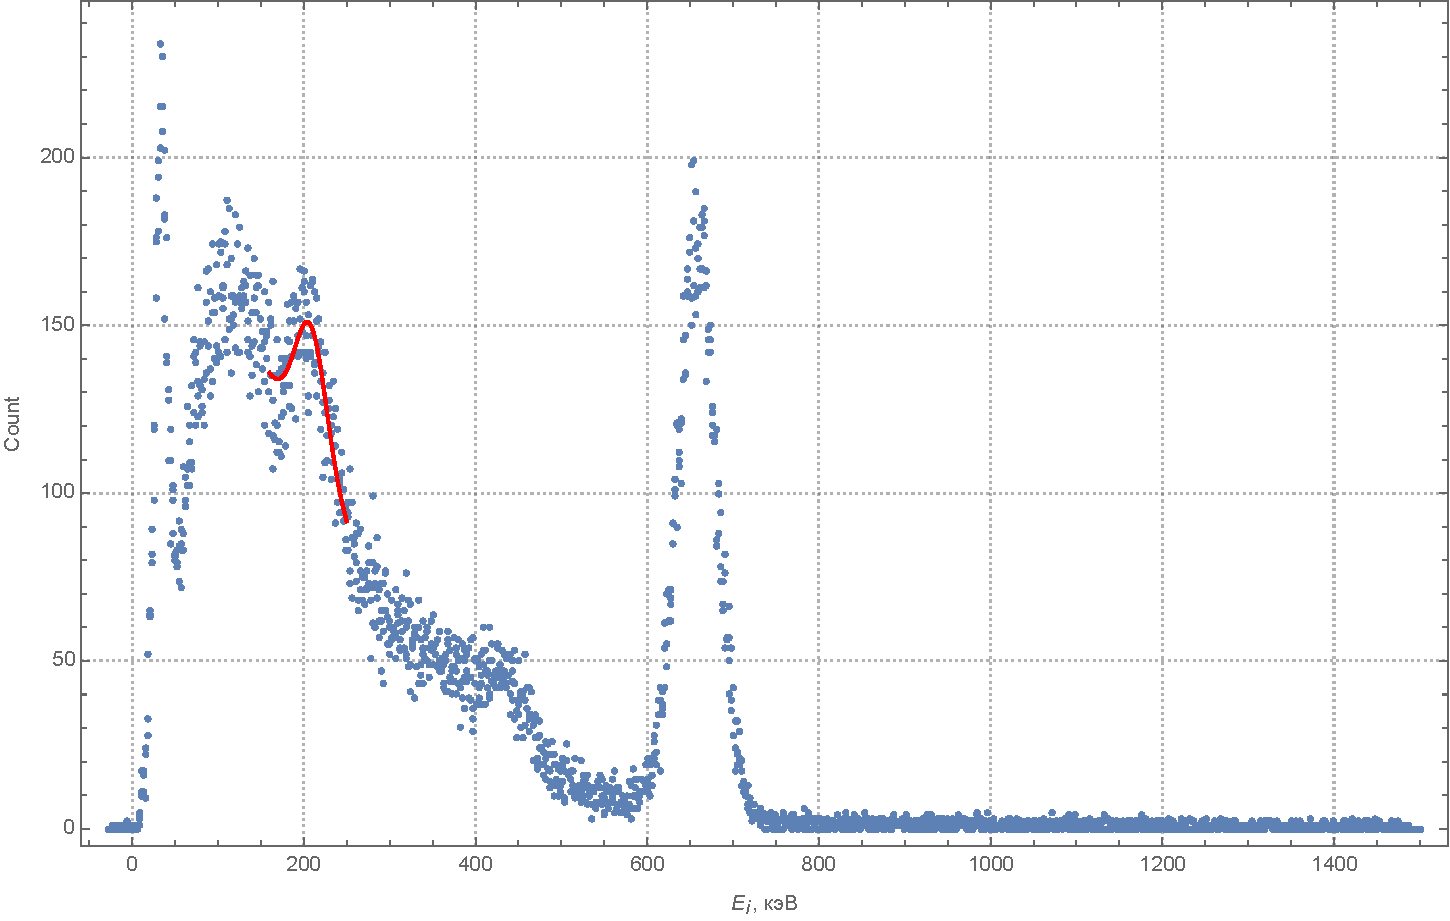
\includegraphics[scale=0.46]{cs137Reverse.pdf}
\caption{Пик обратного рассеяния цезия}
\label{fig:ce137Re}
\end{figure}
\begin{figure}[!htb]
\centering
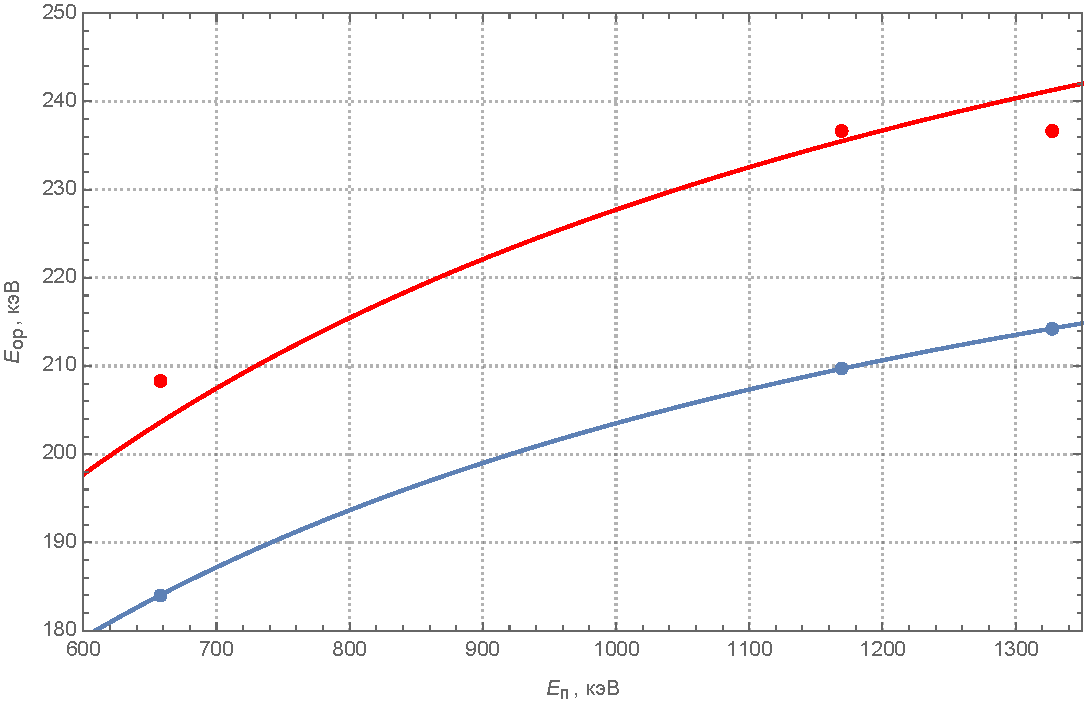
\includegraphics[scale=0.6]{gotPeaks.pdf}
\caption{Пик обратного рассеяния цезия}
\label{fig:gotPeaks}
\end{figure}
\par
В результате экспериментально получили положения пиков рассеяния: для кобальта 236.75 кэВ, для цезия: 208.28 кэВ.\par
Отобразим полученные энергии пиков на графике вместе с расчетными. Для наглядности обозначим расчетные энергии пиков синим цветом, а полученные экспериментальным путем -- красным (рис. \ref{fig:gotPeaks}).\par
Вычислим энергию наблюдаемого характеристического излучения из свинца, служащего защитой спектрометра от внешнего излучения.\par
Пик характеристического излчения хорошо виден в спектрах кобальта, цезия и натрия. Тот факт, что этот же пик наблюдается при измерении фонового излучения подтверждает его происхождение (переизлучение космических лучей свинцом). Энергию характеристического пика найдем из спектра фонового излучения (рис. \ref{fig:background}).
\begin{figure}[!htb]
\centering
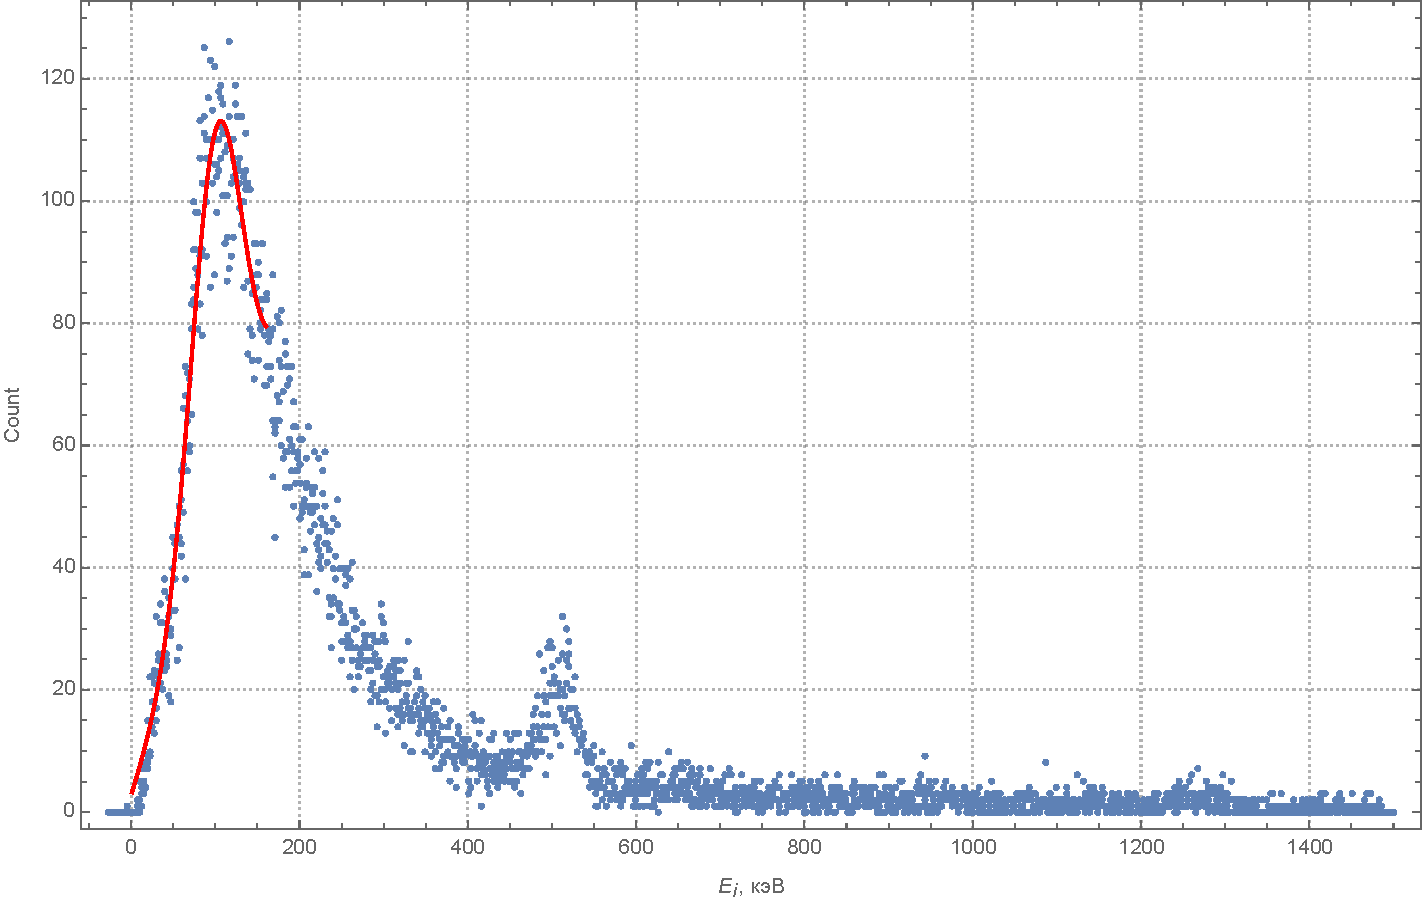
\includegraphics[scale=0.6]{backgroundPb.pdf}
\caption{Фоновое излучение}
\label{fig:background}
\end{figure}
\\
Аппроксимируя пик, получим, что энергия характеристического излучения примерно равна 100.94 кэВ.
\section{Вывод}
В данной работе был разобран принцип работы устройства сцинтиллятора. Также был изучен ряд радиоактивных источников и проверены статистические отношения для разрешающей способности спектрометра.
\end{document}
